%%%%%%%%%%%%%%%%%%%%%%%%%%%%%%%%%%%%%%%%%%%%%%%%%%%%%%%%%%%%%%%%%%%
%                                                                 %
%                            CHAPTER FIVE                         %
%                                                                 %
%%%%%%%%%%%%%%%%%%%%%%%%%%%%%%%%%%%%%%%%%%%%%%%%%%%%%%%%%%%%%%%%%%%

\chapter{MACHINE-READABLE CHANGE LOG}\label{ch:changelog}

\section{Introduction}

Change logs explain the differences between versions; however, they are often only available in human-readable formats.
Readability puts a limit on the length and extent of the log since a human will need to write it.
Manageable change descriptions become difficult with large data sets featuring many changes, or data sets that change often, but these are exactly the data sets which need change logs the most.
Automating the process will allow more data sets to provide change documentation in a timely fashion for data sets.
Encoding the change logs with structured data will provide a means for users to efficiently consume change information.
The additional encoding will inflate the size of a standard change log which becomes an issue with the Noble Gas change log.
This chapter utilizes the Noble Gas and Copper data sets again.

\section{Produce Change Log}

Change logs were generated for both the Noble Gas data set and the Copper data set.
Following the practices of other change logs, the documents present before and after values for comparison which can be seen in Figure \ref{changelog_zoomed}.
\begin{figure}
	\centering
	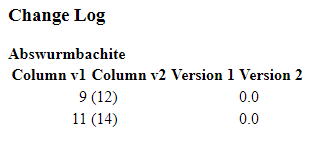
\includegraphics[scale=0.80]{figures/Changelog-zoomed.png}
	\caption{Abswurmbachite entry in the Copper Dataset Change Log}
	\label{changelog_zoomed}
\end{figure}
The partial snapshot of the change log shows that column numbers in the Copper data set also accompany the values to identify the data's location in the spreadsheet.
Very little natural language is used in this change log to regularize the format and improve compatibility with RDFa.
The change logs follow a common format with three sections: Additions, Invalidations, and then Modifications.
The sections may be further grouped by column or row additions.
The division means that changes are not published into the change log as they are found, but instead organized and grouped beforehand.

Employing RDFa means that the document must be written using HTML formatting.
Listing \ref{rdfa_list} shows the text necessary to layout the first four lines of Figure \ref{changelog_zoomed}.
While the content only shows four lines, the underlying markup takes up three and a half times as many lines.
Line 2 states that all following resources will be \textbf{attributes} of Version 1.
Line 3 defines such an \textbf{attribute}.
Lines 5 through 8 define the changes Abswurmbachite undergoes.
Because RDFa allows the statements to be embedded within the content, the triples can appear along with the text they describe.
Lines 11 and 12 define complete triples which do not appear in the visible document.
The lines complete the graph, but must be included in spans because RDFa only allows a single triple within each tag.
Modifying the tags' order so that the spans are unnecessary would cause the visible content to appear in an un-logical order, rendering the document machine-readable but not human-readable.

\begin{lstlisting}[language=HTML, caption=Abswurmbachite RDFa, label=rdfa_list]
<h3>Change Log</h3>
<div about="Version1" rel="vo:hasAttribute">
<div resource="v2:Abswurmbachite" typeof="vo:Attribute">
<span style="font-weight:bold" property="http://www.w3.org/2000/01/rdf-schema#label">Abswurmbachite</span>
<table rel="vo:Undergoes">
<tr  about="ChangeAbswurmbachite12" typeof="vo:Change">
<td align="right" rev="vo:Undergoes" resource="v1:AttributeAbswurmbachite12v1" typeof="vo:Attribute"> 9</td>
<td property="vo:resultsIn" resource="v2:AttributeAbswurmbachite12v2" typeof="vo:Attribute">(12)</td>
<td>          </td>
<td>       0.0</td>
<span about="Version1" property="vo:hasAttribute" resource="v1:AttributeAbswurmbachite12v1"></span>
<span about="Version2" property="vo:hasAttribute" resource="v2:AttributeAbswurmbachite12v2"></span>
</tr>
</table></div></div><br>
\end{lstlisting}

After encountering the limitations of using RDFa to include the versioning graph into the change log, JSON-LD was used.
The new format does not rely on the structure of visible content to determine the syntax triples use to be included in the change log.
Listing \ref{json_list} provides the alternative encoding of the Abswurmbachite entry from RDFa.
The entry is significantly longer, almost three times longer than the RDFa entry and ten times longer than the original visible content.
Instead of including all the data in the beginning or end of the document, each change block is separated into the particular \textit{div} section for that change.
This choice allows consumers to extract pertinent change information without needing to ingest the entire versioning graph.

\begin{lstlisting}[language=HTML, caption=Abswurmbachite JSON-LD, label=json_list]
<h3>Change Log</h3>
<div about="v1:Abswurmbachite">
<span style="font-weight:bold" property="http://www.w3.org/2000/01/rdf-schema#label">Abswurmbachite</span>
<table>
<tr  id="ModifyChangeAbswurmbachite12">
<td align="right"> 9</td>
<td >(12)</td>
<td>          </td>
<td>       0.0</td>
<script type="application/ld+json">
[
{
"@context": "https://orion.tw.rpi.edu/~blee/provdist/GCMD/VO.jsonld", 
"@id": "http://CUdb.com/v1/AttributeAbswurmbachite9", 
"@reverse": {
"hasAttribute": "Version1"
}, 
"@type": "vo:Attribute", 
"label": "Primary", 
"undergoes": "http://orion.tw.rpi.edu/~blee/provdist/CU/DTDI/CUjsonlog.html#ModifyChangeAbswurmbachite12"
}, 
{
"@context": "https://orion.tw.rpi.edu/~blee/provdist/GCMD/VO.jsonld", 
"@id": "http://orion.tw.rpi.edu/~blee/provdist/CU/DTDI/CUjsonlog.html#ModifyChangeAbswurmbachite12", 
"@type": "vo:ModifyChange", 
"resultsIn": "http://CUdb.com/v2/AttributeAbswurmbachite12"
}, 
{
"@context": "https://orion.tw.rpi.edu/~blee/provdist/GCMD/VO.jsonld", 
"@id": "http://CUdb.com/v2/AttributeAbswurmbachite12", 
"@reverse": {
"hasAttribute": "Version2"
}, 
"@type": "vo:Attribute", 
"label": "Primary"
}
]
</script>
</tr>
</table></div><br>
\end{lstlisting}

The encoded change logs struggle with intense document size as summarized in Table \ref{changelog_table}.
The Copper Minerals data set encoded in RDFa is 1.7 MB and JSON-LD is 3.4 MB.
In the Noble Gas data set, the RDFa and JSON-LD change log sizes are 59 and 124 MB, respectively.
The Noble Gas change logs often do not load in a browser.

\begin{table}
	\caption{Sizes of change log encodings.}
	\label{changelog_table}
	\centering
	\begin{tabular}{|c|c|c|c|}
		\hline
		Dataset & No Encoding (MB) & RDFa (MB) & JSON-LD (MB) \\
		\hline
		Copper Minerals & 0.137 & 1.7 & 3.4 \\
		Noble Gas & 5.4 & 59 & 124 \\
		\hline
	\end{tabular}
\end{table}

\section{Change Log Analysis}

The change logs created with RDFa or JSON-LD demonstrates progress towards documents which are both human and machine-readable.
The implementation provides evidence that JSON-LD is better suited to embed a versioning graph into a change log than RDFa.
RDFa suffers limitations since it is constrained by the content's structure.
The \textbf{modify} relation presented in Figure \ref{NobleGraph1} is unbalanced and the right-hand side of ``ChangeCAM00111" links only to the column \textbf{attribute} but not to the corresponding row \textbf{attribute}.
This stems from a mismatch between the model's structure, the order in which data appears in the change log, and the way RDFa links properties together.
Because the row label forms the outermost encapsulation, it cannot instantiate both row identifiers and implicitly link them separately.
To do so would require explicitly instantiating the \textbf{attribute} in a non-visible part of the document, defeating the purpose of using RDFa to implicitly encode the versioning graph into the document.

Both structured data implementations break up the graph across \textbf{attributes} so that individual parts of the graph can be extracted.
The practice of a one-node JSON object is generally helpful for many web applications to load data quickly, but since the change log is not an application, it makes more sense to break up the content.
Changes to individual \textbf{attributes} can be identified using anchors on the web page, then agents need only extract and parse the linked data to these specific entries.
This way, a subgraph of only the pertinent attributes can be created without first ingesting the entire versioning graph.

An unexpected challenge with the change logs is the larger file size and difficulties in loading the Noble Gas data set's JSON-LD change log.
The problem results from needing ten lines to express a single row in the change log.
Noble Gas also had an impressive number of \textbf{modifications}, some of which are shared across all rows in the data set.
Repeated modifications over rows would account for the explosion in entries within the change log.

\section{Summary}

The automated change log generation yielded some unexpected results.
While the data sets differed in both size and structure, the process used to generate the logs followed the same steps.
Because the process to generate versioning graphs already separates changes into groups, the change log is organized into similar categories.
Much of the data visible in the change log does not explicitly appear in the model such as the pre and post-values.

The human-readable presentation defines the structure which tags in the change log must take since maintaining human-readability is desired.
The structure then determines the order in which linked data statements must appear in the log to encode the graph with RDFa.
The ordering creates limitations on how strictly the encoded graph adheres to the specification from Chapter \ref{ch:model}.
While construction of the change log is automated, encoding through RDFa significantly reduces the source HTML readability.
In other applications using RDFa, the triples describe and link the text encapsulated by HTML tags.
The versioning graph exclusively ignores the marked up content and links together tags or explicitly defines full triples in span tags.

Change logs are much less restricted when encoded using JSON-LD rather than RDFa.
The encoding format pulls the graph out of the attributes where they do not interact with content and into a separate script section.
The method causes a drastic expansion per change in necessary text.
The decision to divide up JSON-LD objects by the row in the change log they describe likely contributes significantly to the overhead necessary for the encoding.
The division was made with the forethought that change log consumers may desire to only ingest specific subgraphs of the versioning graph.
Separated JSON-LD objects will likely need to be merged in the future to save space for data sets with many changes.

The resulting logs end up very large and sometimes do not load in a browser.
Reassuringly, both data sets displayed the same space usage complexity with RDFa being ten times the plain text size and JSON-LD twice the size of a change long in RDFa.
The relationship unfortunately means that a JSON-LD change log, with more readable source code, is twenty times the size of a plain text change log.
The Copper data set's logs were reasonably responsive, displaying in seconds, but the Noble Gas's change log did not.
In order to retain usability, there will need to be methods optimizing change log structure or representation.